\section{Sink KV}
\label{sec:app-sink-kv}


\begin{figure*}[b]
  \centering
  \begin{subfigure}[t]{0.45\columnwidth}
    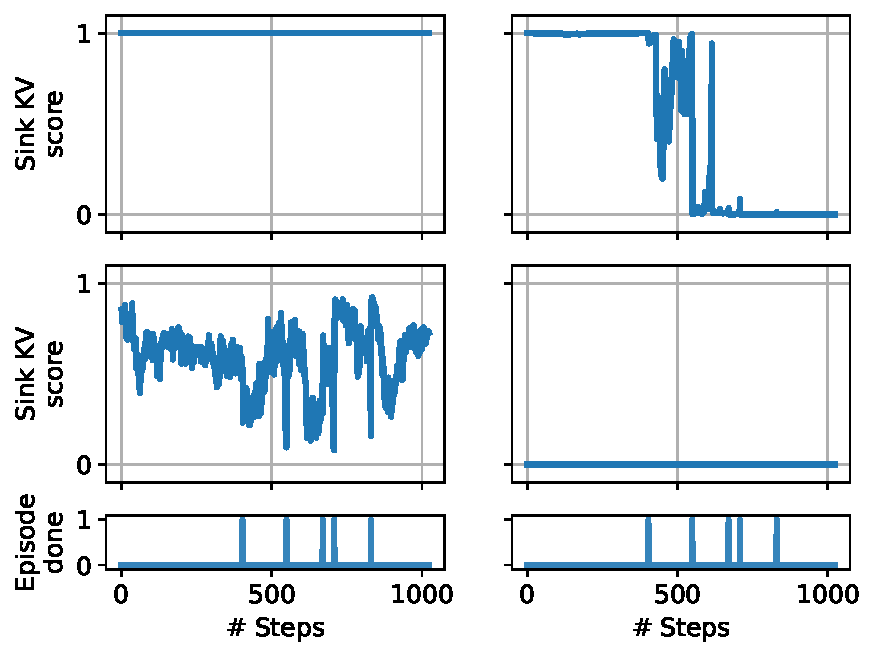
\includegraphics[width=\textwidth]{figures/results/sink_kv_patterns.pdf}
    \caption{Different patterns of Sink $KV$ scores  for 1k input tokens.}
    \label{fig:app-sink-kv-scores}
  \end{subfigure}
  \begin{subfigure}[t]{0.45\columnwidth}
    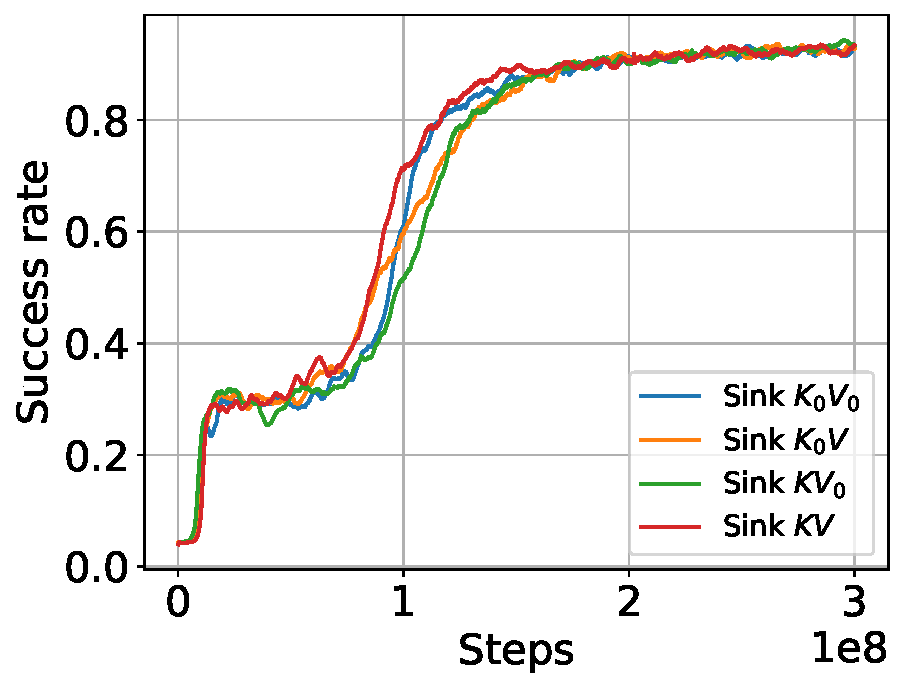
\includegraphics[width=\textwidth]{figures/results/sinktok_exps_variants.pdf}
    \caption{The learning curve for the Sink $KV$ variants.}
    \label{fig:app-sink-kv-variants}
  \end{subfigure}
  \caption{
    Sink $KV$ analysis.
  }
  \label{fig:sink-kv-analysis}
\end{figure*}


We introduce Sink $KV$, a modification to the attention calculation in the attention layers.
We first describe the vanilla attention \cite{vaswani2023attention}, the issue and the motivation to find a solution. Then we discuss the proposed solutions and introduce the \sinkv technique. Finally, we anlayze different variants of \sinkv.


\subsection{Motivation}
The vanilla attention is the component responsible for the interaction between the tokens in the sequence. The output for each token is calculated by weighting the value of all tokens.
The input to the attention layer is the embeddings of the input tokens $E\in \mathbb{R}^{n\times d}$ where $n$ is the number of input tokens and $d$ is the dimension of the embeddings.

First the embeddings $E$ are linearly projected to the Key $K$, Value $V$ and Query $Q$. Then the attention scores are calculated using $S=\text{Softmax}(QK^T/\sqrt{d_k})$ where $d_k$ is the dimensions of the keys. The output $A$ is calculated as a weighted sum of the values $V$,  $A=SV$. 

The calculation of the attentions scores $S$ using the $\text{Softmax}$ forces the tokens to attend to values $V$, even if all available values do not hold any useful information, since the sum of the scores is 1 \citep{off_by_one_softmax}. This is especially harmful in cases where the task requires exploration. As the agent explores more, a more useful information may appear in the sequence. If the agent is forced to attend to low information tokens at the beginning of the exploration, it will introduce noise to the attention layers.



\subsection{Solutions}
\label{sec:app-sinkkv-solutions}

Softmax One from \cite{off_by_one_softmax} addresses this issue by adding $1$ to the denominator of the $\text{Softmax}$, $\text{Softmax}_1(x_i) :=\exp(x_i)/(1+\sum_j{\exp(x_j)})$, which is equivalent to having a token with $k=0$ and $v=0$. This gives the model the ability to have 0 attention score to all tokens, we refer to Softmax One as Sink $K_0V_0$.

Sink tokens from \cite{xiao2023efficient} are another approach to address the same issue by prepending learnable tokens to the input tokens $E=[E_s \circ E_{input}]$ where $E$ is the input embedding to the model and $[A\circ B]$ indicates concatenation along the sequence dimension of the $A$ and $B$ matrices .

\sinkv is a generalization of both approaches. It modifies the attention layer by adding a learnable Key $K_s\in\mathbb{R}^{n\times d_k}$ and values $V_s\in\mathbb{R}^{n\times d}$. In each attention layer, we simply prepend the learnable $K_s$ and $V_s$ to the vanilla keys $K_v$ and values $V_v$ to get the $K=[K_s \circ K_v]$ and $V=[V_s \circ V_v]$ used to calculate the attention scores then the attention output. 

In the case $K_s=0$ and $V_s=0$, \sinkv becomes equivalent to Softmax One. It can also learn the same $K$s and $V$s corresponding to the Sink Token since our model is casual and the processing of the Sink Token is not affected by the remaining sequence.

\subsection{\sinkv variants}
We tried a variant of \sinkv where the either the Value or the Key is set to 0, referred to as Sink $KV_0$ and Sink $K_0V$ respectively. All variants perform similarly in terms of the success rate as shown in \Cref{fig:app-sink-kv-variants}.


\Cref{fig:app-sink-kv-scores} shows different patterns the model uses the Sink $KV_0$. The model can assign all attention scores to the Sink $KV_0$, which yields a zero output for the attention head, or assign variable scores at different time in the generation. For example, one the attention heads is turned off during the 1st episode of the trial by assigning all attention score to the Sink $KV_0$ then eventually move the attention to the input tokens in the new episodes. The model is also able to ignore the Sink $KV_0$ by assigning it 0 attention scores as shown in the figure. 
